\chapter{Detailanalyse der Aufgabenstellung}
In der Detailanalyse der Aufgabenstellungen formuliere ich die zu bewältigenden
Aufgaben und deren erwartete Resultate aus.

\section{Aufgaben und Resultate}
\subsubsection{Ist-Situation im Bereich Projektablauf der allink.creative erfassen}
Es soll eine Beschreibung des aktuellen Projektablaufes der allink erarbeitet
und möglichst vollständig alle heutigen Prozessschritte dargestellt und die Vor- 
und Nachteile des Projektablaufes aufgezeigt werden. Hinzu kommt die darin verwendete Software und
deren Einsatzzweck.
\\\\
\underline{Erwartete Resultate}

\begin{description}
    \item[R1] Beschreibung der Ist-Situation im Bereich Projektablauf
    \item[R2] Übersicht der bestehenden Software beim Auftraggeber
\end{description}

\subsubsection{Kennzahlen definieren, die in Zukunft auf Projektebene gemessen werden sollen}
Zusammen mit dem Auftraggeber sollen Voraussetzungen, unteranderem Kennzahlen,
definiert werden, die bei der Erarbeitung des neuen Projektablaufes berücksichtig
werden müssen. 
\\\\
\underline{Erwartete Resultate}

\begin{description}
    \item[R3] Anforderungen an den neuen Prozess inkl. Kennzahlen, die auf 
        Projektebene gemessen werden sollen
\end{description}
  
\subsubsection{Eine Recherche der Prozesse in ähnlich funktionierenden KMUs durchführen}
Der Studierende soll in Gesprächen mit anderen KMUs recherchieren, was Agenturen
mit ähnlichen Voraussetzungen und Herausforderungen wie allink für Projektabläufe
und Hilfsmittel verwenden.
\\\\
\underline{Erwartete Resultate}

Die Informationen aus den Recherchen sollen in den Lösungsvorschlag eingearbeitet
und berücksichtigt werden.

\subsubsection{Neue Prozesse definieren und bestehende, sofern sinnvoll, überarbeiten}
Anhand den bis dahin gewonnen Erkenntnissen soll der bestehende Projektablauf
überarbeitet und neu definiert werden. Dazu arbeitet der Studierende eng mit
dem Auftraggeber zusammen, damit sichergestellt ist, dass eine in der Realität
umsetzbare Lösung definiert wird.
\\\\
\underline{Erwartete Resultate}

\begin{description}
    \item[R4] Konzept des neuen und überarbeiteten Prozesses
    \item[R5] Übersicht der bestehenden Software in der neuen Prozesslandschaft
    \item[R6] Softwareempfehlungen für die komplette Prozessabbildung
\end{description}

\subsubsection{Evaluation von IT-Lösungen, die diese Prozesse möglichst passend 
    für den Auftraggeber abbilden und die definierten Kennzahlen generieren können}
Sofern die bestehende Software des Auftraggebers nicht ausreicht um den neuen
Projektablauf im Unternehmen umzusetzen, soll der Studierende alternative 
Lösungen evaluieren. Darin können auch selbst umzusetzende Tools empfohlen 
werden, sofern der Aufwand für dessen Entwicklung gerechtfertigt ist.
\\\\
\underline{Erwartete Resultate}

\begin{description}
    \item[R7] ``Make or Buy''-Entscheid mit dem Auftraggeber
\end{description}

\section{Aufwandschätzung}
Aufgrund den Anforderungen an eine Diplomarbeit und aus der Aufgabenstellung
ergeben sich für mich Arbeitspakete, die ich in eine Planungs- und Umsetzungsphase
der Diplomarbeit unterteile. Auch versuche ich den Aufwand der einzelnen
Arbeitspaketen in Stunden zu schätzen und diese dann in eine realistische 
Projektplanung einfliessen zu lassen.

\subsection{Planungsphase}
Die Arbeitspakete, die vor der Freigabe der Diplomarbeit erbracht werden müssen,
sind in Stunden geschätzt und in der Tabellen \ref{tab:auwand_planungsphase} 
aufgelistet.

\begin{table}[htbp]
\begin{center}
    \begin{tabular}{llc}
        \toprule & \textbf{Arbeitspaket} & \textbf{Aufwand in Stunden} \\
        \midrule \textbf{P1} & Thema evaluieren & 16 \\
        \midrule \textbf{P2} & Aufgabenstellung ausarbeiten & 20 \\
        \midrule \textbf{P3} & Betreuer finden & 16 \\
        \midrule \textbf{P4} & Kick-Off vorbereiten & 12 \\
        \bottomrule & \textbf{Total Stunden} & \textbf{64} \\
        \bottomrule
    \end{tabular}
    \caption{Aufwandschätzung der Arbeitspakete der Planungsphase}
    \label{tab:auwand_planungsphase}
\end{center}
\end{table}

\subsection{Umsetzungsphase}
Die Arbeitspakete, die während der Diplomarbeit erbracht werden müssen, sind
in Stunden geschätzt und in der Tabelle \ref{tab:aufwand_umsetzungsphase}
aufgelistet.

\begin{table}[htbp]
\begin{center}
    \begin{tabular}{llc}
        \toprule & \textbf{Arbeitspaket} & \textbf{Aufwand in Stunden} \\
        \midrule \textbf{P5} & Ist-Situation erfassen & 40 \\
        \midrule \textbf{P6} & Kennzahlen definieren & 28 \\
        \midrule \textbf{P7} & Review vorbereiten & 12 \\
        \midrule \textbf{P8} & Prozesse definieren und überarbeiten & 44 \\
        \midrule \textbf{P9} & Evaluation von IT Lösungen & 28 \\
        \midrule \textbf{P10} & Abschluss Arbeit & 16 \\
        \midrule \textbf{P11} & Druckauftrag & 12 \\
        \midrule \textbf{P12} & Vorbereitung Präsentation & 16 \\
        \bottomrule & \textbf{Total Stunden} & \textbf{196} \\
        \bottomrule
    \end{tabular}
    \caption{Aufwandschätzung der Arbeitspakete der Umsetzungsphase}
    \label{tab:aufwand_umsetzungsphase}
\end{center}
\end{table}

\chapter{Projektadministration}
\section{Projektplan}
Den provisorischen Projektplan erstelle ich aufgrund den geschätzten Aufwände
und den vorgegebenen Terminen der HSZ-T. Die gewählten Termine der Meilensteine
``Abgabe Diplomarbeit'' und ``Präsentation Diplomarbeit'' sind meine Wunschtermine
und noch nicht offiziell bestätigt.

Das Total der zu bewältigenden und geschätzten Stunden beläuft sich 
auf 260 Stunden. Diese versuche ich möglichst realistisch über den mir noch
zur Verfügung stehenden Zeitraum zu verteilen. Dies habe ich mit Hilfe der 
Projektplanungs-Software Merlin\footnote{Website von Merlin, \url{http://www.projectwizards.net/de/merlin/}} 
erstellt und eine Übersicht ist in der unten stehenden Grafik \ref{pic:projektplan} 
dargestellt.

\begin{figure}[htbp]
\begin{center}
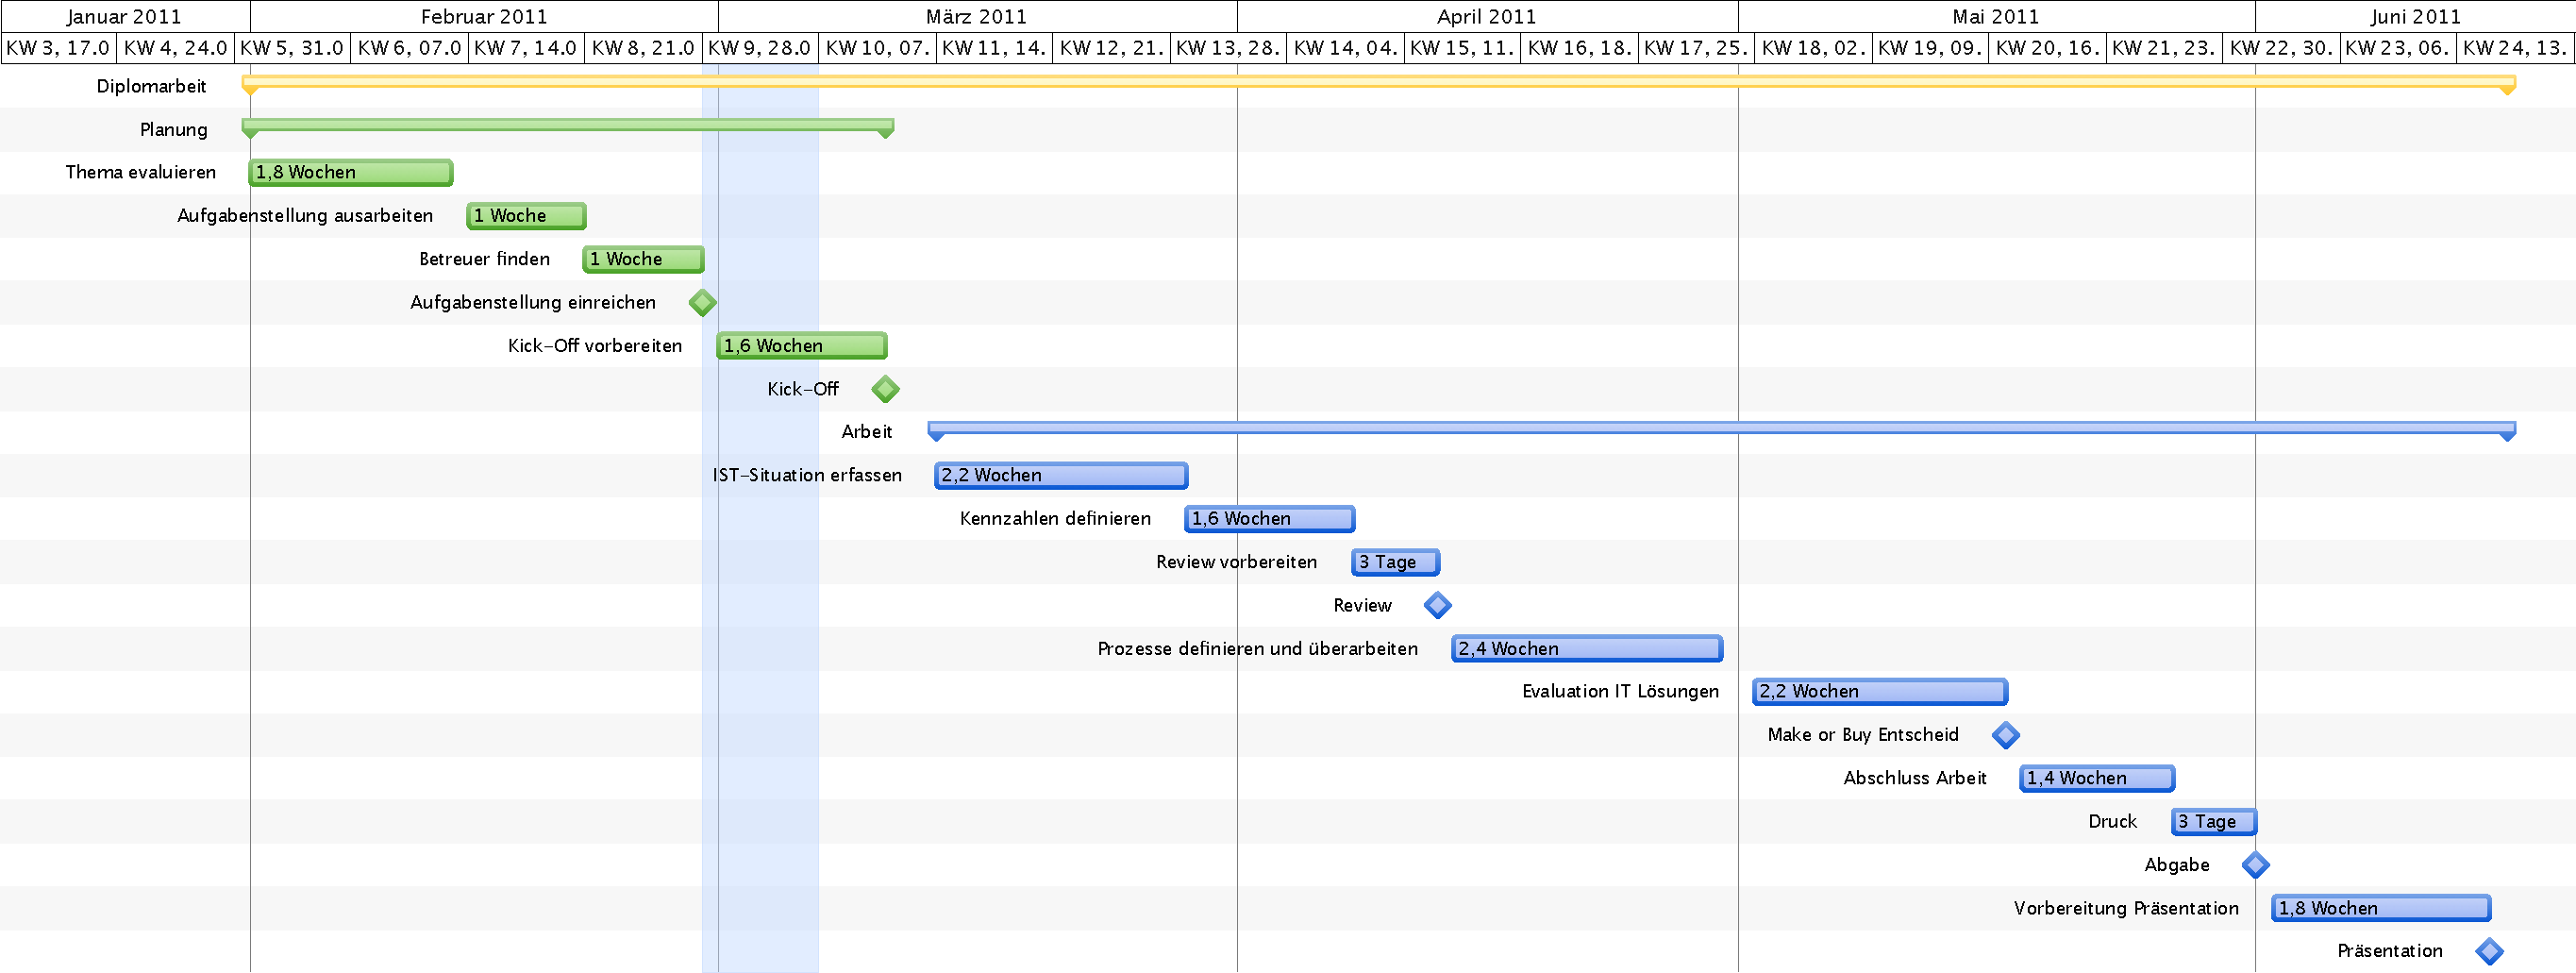
\includegraphics[width=1\textwidth,angle=0]{./bilder/anhang/projektplanung.pdf}
\caption{Projektplan der Diplomarbeit aus Merlin}
\label{pic:projektplan}
\end{center}
\end{figure}

Ich bin mir bewusst, dass es eine eher optimistische Projektplanung ist. Jedoch
steht mir, aus administrativen Gründen der HSZ-T, nur noch dieser Zeitraum für
die Durchführung der Diplomarbeit übrig um mein Studium erfolgreich abschliessen
zu können. Trotz der optimistischen Planung bin ich zuversichtlich, diese
im gegebenen Zeitrahmen umsetzen und abschliessen zu können.

Zum Zeitpunkt des Designreviews werde ich anhand des bisherigen Projektverlaufes
die Situation neu beurteilen und, wenn nötig, die Planung überdenken und 
gegebenenfalls anpassen.

\section{Termine}
In der Tablle \ref{tab:termine_diplomarbeit} sind alle Termine, die sich aus 
dem Projektplan, den bekannten Terminen und Wunschterminen ergeben, in chronologischer
Reihenfolge ihrer Durchführung aufgelistet.

Zusätzlich habe ich sie mit den abhängenden Arbeitspaketen
und Resultaten ergänzt, die zum Zeitpunkt des Termins vorhanden und erfüllt
sein sollten.

\begin{table}[htbp]
\begin{center}
    \begin{tabular}{llll}
        \toprule & & \multicolumn{2}{c}{\textbf{Abhängende}} \\
        \textbf{Datum} & \textbf{Termin} & \textbf{Arbeitspakete} & \textbf{Resultate} \\
        \midrule 28.02.2011 & Aufgabenstellung einreichen & P1, P2, P3 & - \\
        \midrule 11.03.2011 & Kick-Off Meeting & P4 & -\\
        \midrule 13.04.2011 & Review Termin & P5, P6, P7 & R1, R2, R3 \\
        \midrule 17.05.2011 & ``Make or Buy''-Entscheid & P8, P9 & R4, R5, R6 \\
        \midrule 01.06.2011 & Abgabe Diplomarbeit & P10, P11 & R7 \\
        \midrule 15.06.2011 & Präsentation Diplomarbeit & P12 & - \\
        \bottomrule
    \end{tabular}
    \caption{Auflistung der Termine der Diplomarbeit}
    \label{tab:termine_diplomarbeit}
\end{center}
\end{table}

\section{Versionsverwaltung}
Zur besseren Nachvollziehbarkeit meiner Diplomarbeit führe ich seit Beginn an
ein Repository mit git\footnote{Freie Software zur Versionsverwaltung von Dateien,
\url{http://git-scm.com/}} und ein ausführliches Arbeitsprotokoll als Wikipage.
Meinen aktuellen Stand inklusive aller Unterlagen veröffentliche ich auf der 
Plattform github\footnote{Hosting Dienst, \url{https://github.com/}}. Diese 
Informationen sind öffentlich verfügbar und für jedermann unter folgenden 
Adressen zugänglich:

\subsection{git Repository}
\url{https://github.com/sspross/diplomarbeit}

\subsection{Wiki}
\url{https://github.com/sspross/diplomarbeit/wiki}

\subsection{Arbeitsprotokoll}
\url{https://github.com/sspross/diplomarbeit/wiki/arbeitsprotokoll}

\section{Erreichte Ziele}
In der nachfolgenden Tabelle \ref{tab:erreichte_ziele} sind alle Ziele gemäss 
den erwarteten Resultaten der Aufgabenstellung aufgelistet. Alle 
erwarteten Ziele wurden erreicht.

\begin{table}[htbp]
\begin{center}
    \begin{tabular}{p{10cm}lcl}
        \toprule \textbf{Ziel} & \textbf{Resultat} & \textbf{Stand} \\
        \midrule Die Ist-Situation im Bereich Projektablauf der allink.creative
            ist beschrieben und abgebildet. & R1 & erfüllt \\
        \midrule Eine Übersicht über die bestehende Software bei allink.creative
            wurde erstellt. & R2 & erfüllt \\
        \midrule Die Anforderungen an den neuen Prozess inkl. Kennzahlen, die auf 
            Projektebene gemessen werden sollen, wurden definiert. & R3 
            & erfüllt \\
        \midrule Das Konzept des neuen und überarbeiteten Prozesses ist 
            vorhanden. & R4 & erfüllt \\
        \midrule Eine Übersicht über die bestehende Software bei allink.creative
            in der neuen Prozesslandschaft wurde erstellt. & R5 & erfüllt \\
        \midrule Eine Softwareempfehlung für die komplette Prozessabbildung
            wurde erstellt und begründet. & R6 & erfüllt \\
        \midrule Ein ``Make or Buy''-Entscheid wurde mit dem Auftraggeber 
            getroffen und festgehalten. & R7 & erfüllt \\
        \bottomrule
    \end{tabular}
    \caption{Auflistung der erwarteten Resultate mit Stand der Erfüllung}
    \label{tab:erreichte_ziele}
\end{center}
\end{table}